\thispagestyle{empty}
% \section*{Eidesstattliche Versicherung}
% Ich versichere hiermit an Eides statt, dass ich die vorliegende Abschlussarbeit mit dem Titel \enquote{\thetitle} selbstständig und ohne unzulässige fremde Hilfe erbracht habe.
% Ich habe keine anderen als die angegebenen Quellen und Hilfsmittel benutzt, sowie wörtliche und sinngemäße Zitate kenntlich gemacht.
% Die Arbeit hat in gleicher oder ähnlicher Form noch keiner Prüfungsbehörde vorgelegen.
%
% \vspace*{1cm}\noindent
% \begin{center}
%   \begin{tabular}{@{}p{0.4\textwidth}@{\hspace{0.15\textwidth}}p{0.4\textwidth}@{}}
%   \rule{\linewidth}{0.25pt}& \rule{\linewidth}{0.25pt}\\
%   Ort, Datum & Unterschrift
%   \end{tabular}
% \end{center}
%
% \subsection*{Belehrung}
% Wer vorsätzlich gegen eine die Täuschung über Prüfungsleistungen betreffende Regelung einer Hochschulprüfungsordnung verstößt, handelt ordnungswidrig.
% Die Ordnungswidrigkeit kann mit einer Geldbuße von bis zu \SI[round-mode=places, round-precision=2]{50000}{€} geahndet werden.
% Zuständige Verwaltungsbehörde für die Verfolgung und Ahndung von Ordnungswidrigkeiten ist der Kanzler/die Kanzlerin der Technischen Universität Dortmund.
% Im Falle eines mehrfachen oder sonstigen schwerwiegenden Täuschungsversuches kann der Prüfling zudem exmatrikuliert werden \mbox{(\S\,63 Abs. 5 Hochschulgesetz --HG--).}
%
% Die Abgabe einer falschen Versicherung an Eides statt wird mit Freiheitsstrafe bis zu 3 Jahren oder mit Geldstrafe bestraft.
%
% Die Technische Universität Dortmund wird ggf.\ elektronische Vergleichswerkzeuge (wie z.\,B.\ die Software \enquote{turnitin}) zur Überprüfung von Ordnungswidrigkeiten in Prüfungsverfahren nutzen. \\[\baselineskip]
%
% \noindent Die oben stehende Belehrung habe ich zur Kenntnis genommen.\\[1cm]
% \begin{center}
% \begin{tabular}{@{}p{0.4\textwidth}@{\hspace{0.15\textwidth}}p{0.4\textwidth}@{}}
% \rule{\linewidth}{0.25pt}& \rule{\linewidth}{0.25pt}\\
% Ort, Datum & Unterschrift
% \end{tabular}
% \end{center}

\begin{figure}
  \centering
  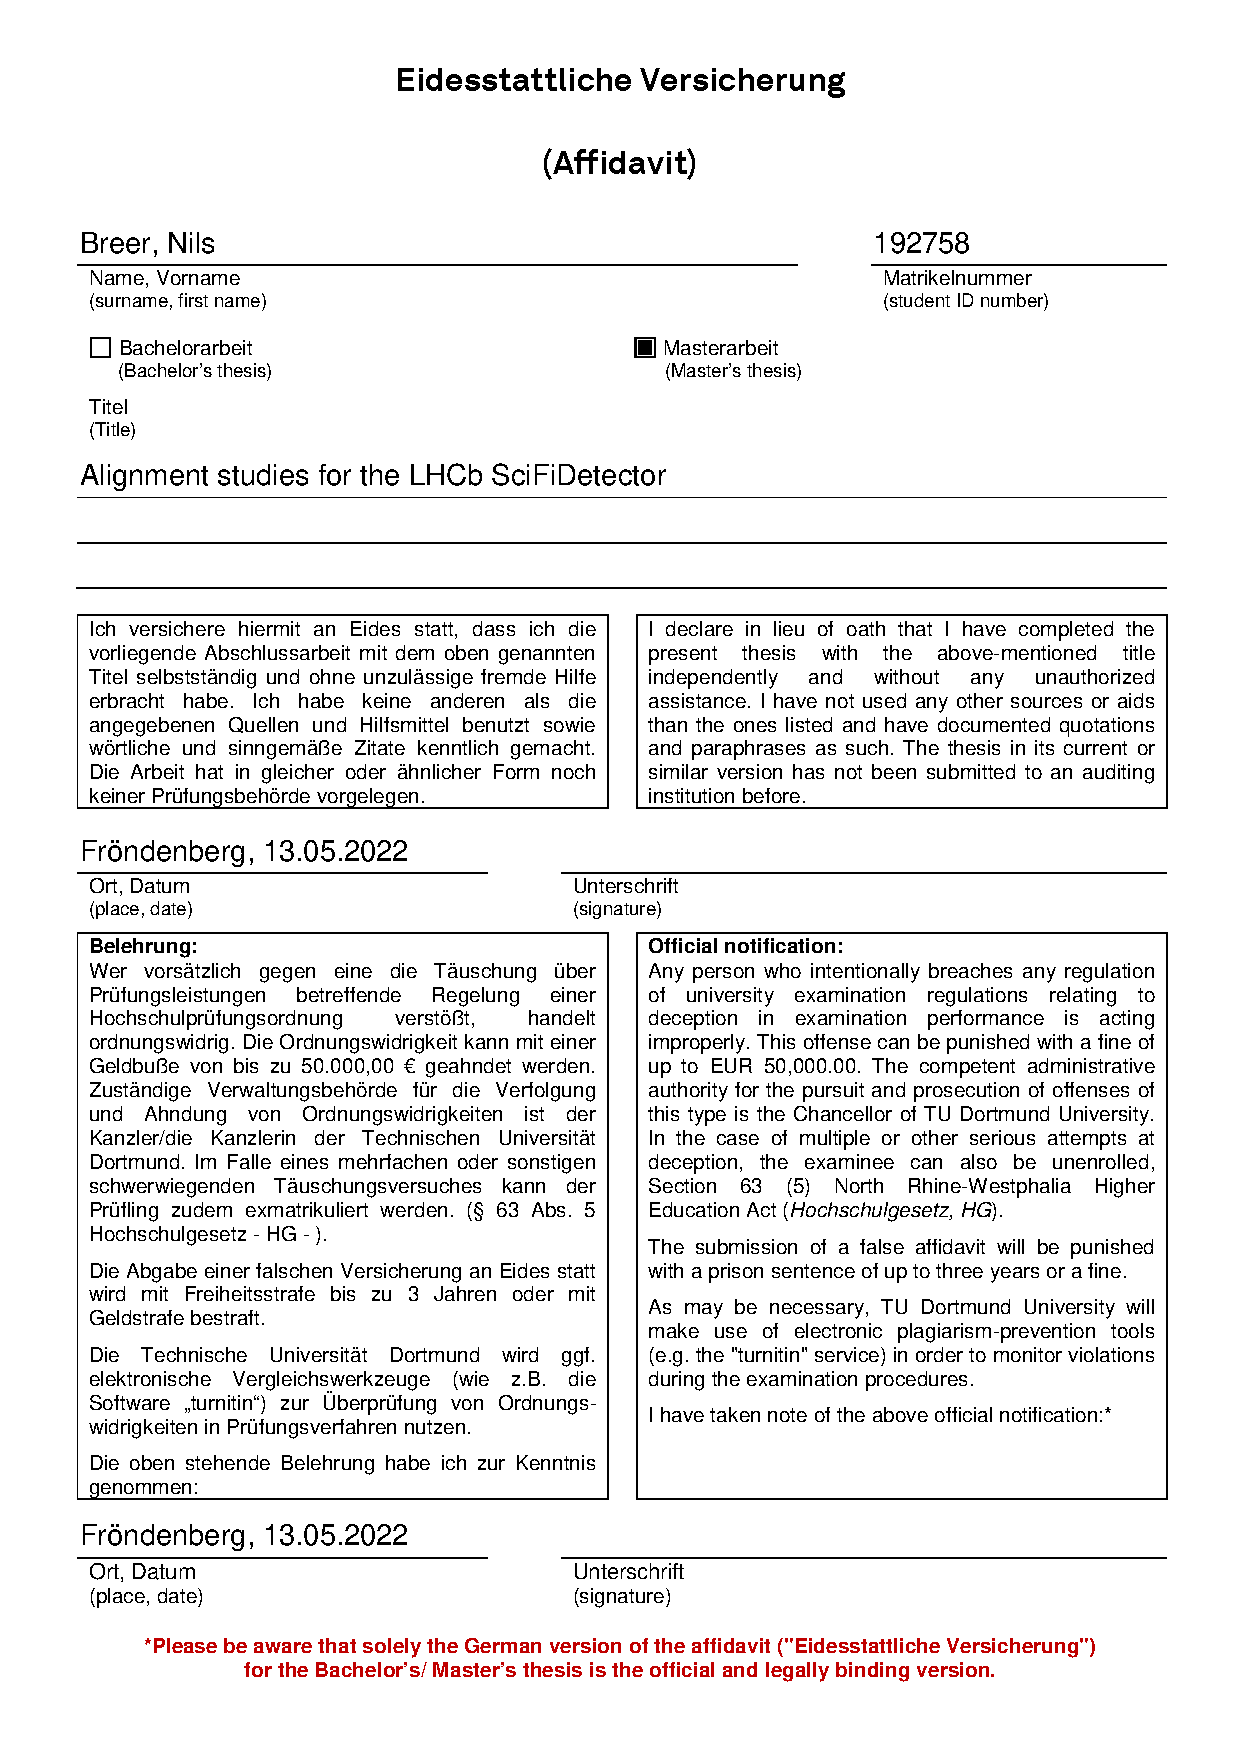
\includegraphics[width=\textwidth]{Eidesstattliche_Versicherung.pdf}
\end{figure}
